%  LaTeX support: latex@mdpi.com
%  For support, please attach all files needed for compiling as well as the log file, and specify your operating system, LaTeX version, and LaTeX editor.

%=================================================================
\documentclass[sensors,apajournal,article,submit,moreauthors]{Definitions/mdpi}
% For posting an early version of this manuscript as a preprint, you may use "preprints" as the journal.

%=================================================================
% MDPI internal commands - do not modify
\firstpage{1}
\makeatletter
\setcounter{page}{\@firstpage}
\makeatother
\pubvolume{1}
\issuenum{1}
\articlenumber{0}
\pubyear{2026}
\copyrightyear{2026}
\datereceived{}
\daterevised{}
\dateaccepted{}
\datepublished{}

%=================================================================
% Title
\Title{A Four-Tier Stakeholder-Specific Explainable AI Framework for Trustworthy Network Intrusion Detection}

% Authors
% ORCIDs verified via ORCID public API (https://pub.orcid.org/v3.0/) and OpenAlex
% E (Abdelrahim) confirmed as co-author via Youssef Saleh's co-authored paper
% D (Ibrahim) is at UIdaho per the original thesis committee but has no public ORCID on file
\newcommand{\orcidauthorA}{0009-0008-3742-1358}  % Youssef Saleh (University of Idaho)
\newcommand{\orcidauthorB}{0000-0003-1241-2750}  % Frederick Sheldon (University of Idaho, Computer Science, Professor)
\newcommand{\orcidauthorC}{0000-0001-5572-4303}  % Terrence Soule (University of Idaho, Computer Science, Professor)
\newcommand{\orcidauthorD}{0000-0002-3039-4560}  % Ahmed A. Ibrahim (University of Idaho, Civil and Environmental Engineering, Professor)
\newcommand{\orcidauthorE}{0000-0001-9756-554X}  % Ahmed Abdel-Rahim (University of Idaho)

\Author{Youssef Saleh $^{1}$\orcidA{}, Frederick Sheldon $^{2,}$*\orcidB{}, Terrence Soule $^{2}$\orcidC{}, Ahmed Ibrahim $^{2}$\orcidD{} and Ahmed Abdelrahim $^{2}$\orcidE{}}

\AuthorNames{Youssef Saleh, Frederick Sheldon, Terrence Soule, Ahmed Ibrahim and Ahmed Abdelrahim}

% Affiliations
\address{%
$^{1}$ \quad Department of Computer Science, University of Idaho, Moscow, ID 83844, USA; saleh@uidaho.edu\\
$^{2}$ \quad Department of Computer Science, University of Idaho, Moscow, ID 83844, USA; sheldon@uidaho.edu (F.S.)}

% Contact
\corres{Correspondence: Frederick Sheldon, Department of Computer Science, University of Idaho, Moscow, ID 83844, USA. Email: sheldon@uidaho.edu}

% Abstract (single paragraph, ~200 words)
\abstract{Modern Intrusion Detection Systems (IDS)~\citep{khraisat2019survey,mahdavifar2019application,ferrag2020deep} increasingly rely on deep learning classifiers whose black-box behavior erodes operator trust~\citep{adadi2018peeking,amann2020explainability}. We present a \mbox{stakeholder-specific} Explainable AI (XAI) framework for network packet analysis that produces four \mbox{role-tailored} explanations of every detection: one each for a Security Analyst, an IT Manager, a Software Developer, and a Compliance Officer. The architecture combines a CNN-LSTM hybrid classifier~\citep{hochreiter1997long,chollet2017xception} with SHAP and LIME~\citep{lundberg2017unified,ribeiro2016why} for global and local feature attribution, then feeds these attributions into a locally deployed, GGUF-quantized Mistral-7B large language model (LLM)~\citep{touvron2023llama,brown2020language} that emits structured natural-language narratives. Evaluated on the UNSW-NB15 and NSL-KDD benchmark datasets, the CNN-LSTM classifier achieved 96.76\% accuracy with an F1-score of 0.9675; the XAI layer attained a sufficiency metric of 0.9390 and a SHAP-LIME \mbox{top-3 agreement} of 12.2\%. The LLM pipeline produced syntactically clean, semantically grounded explanations with 5.5\% estimated semantic hallucination. By aligning explanation depth and framing with each stakeholder's decision context, the framework restores the evidence chain that operators require to act on automated security output.}

% Keywords
\keyword{Explainable AI; Network Intrusion Detection; Deep Learning; CNN-LSTM; SHAP; LIME; Large Language Models; Cybersecurity; Stakeholder-Specific Explanations}

%=================================================================
%=================================================================
% Hyphenation control
%hyphenation{} does NOT work in MDPI class - using mbox for compound words instead

\begin{document}
\section{Introduction}

The accelerating sophistication of network attacks has outpaced the evolution of detection systems that human operators can understand and trust~\citep{apruzzese2020deep,khraisat2019survey,vinayakumar2019deep}. Signature-based \mbox{intrusion detection} fails on novel attacks; supervised deep learning~\citep{vinayakumar2019deep,ferrag2020deep} fills that gap, but introduces a new one: predictions arrive without explanations~\citep{adadi2018peeking,bhatt2020explainable,goodfellow2014explaining}. Security analysts cannot triage alerts whose reasoning is opaque~\citep{apruzzese2020deep}; managers cannot allocate budget on uninterpretable risk scores; developers cannot act on alerts that do not map to code; compliance officers cannot file audit records without an evidence chain~\citep{ferrag2020deep}. This paper addresses that gap directly.

We propose a four-tier Explainable AI (XAI) framework that produces \mbox{stakeholder-specific} explanations of every detection. Tier 1 normalizes packet features across heterogeneous datasets; Tier 2 runs a CNN-LSTM hybrid classifier that achieves 96.76\% accuracy on the combined UNSW-NB15 and NSL-KDD benchmark; Tier 3 adds SHAP and LIME attribution; Tier 4 routes those attributions through a locally deployed Mistral-7B LLM to generate \mbox{role-tailored} narratives. The result is one detection, four \mbox{stakeholder-grounded} explanations.

The contributions of this work are:
\begin{itemize}
\item A unified four-tier pipeline that integrates packet classification, dual-XAI attribution, and LLM-based natural-language explanation in a single deployable system.
\item A \mbox{stakeholder-conditioned} prompt template that generates semantically and structurally distinct narratives for four operational roles from a shared XAI foundation.
\item A comprehensive evaluation protocol combining sufficiency, comprehensiveness, perturbation-based fidelity, and SHAP-LIME agreement, plus a 20-instance rubric-based LLM evaluation with role-specific differentiation.
\item Empirical demonstration of faithful explanations on UNSW-NB15 and NSL-KDD with a 100\% generation success rate and 5.5\% estimated semantic hallucination.
\end{itemize}

\section{Materials and Methods}

\subsection{Datasets and Preprocessing}

We evaluated the framework on two widely used IDS benchmarks: UNSW-NB15~\citep{moustafa2015unsw} (2015 traffic) and NSL-KDD~\citep{tavallaee2009detailed} (refined KDD-1998). These benchmarks are widely adopted in the IDS literature~\citep{khraisat2019survey,mahdavifar2019application}. To enable \mbox{cross-dataset} training we constructed a 37-feature canonical schema representing the intersection of both schemas. Numeric features undergo Z-score standardization; categorical features (protocol type, service, flag) are one-hot encoded. The preprocessing module (data\_preprocessing.py) implements fuzzy column matching to map dataset-specific names to the canonical schema, validated by a schema-drift test suite.

Class imbalance is addressed with SMOTE~\citep{chawla2002smote} oversampling at a 0.6 ratio, applied only to the training split to avoid leakage. Class-weighted binary cross-entropy with positive weight 2.5 compensates for the residual imbalance. Label smoothing ($\epsilon = 0.05$) prevents overconfident predictions that would distort downstream SHAP attributions.

\subsection{Framework Architecture}

The framework is organized into four sequential tiers, each handling a distinct stage of the \mbox{intrusion detection} pipeline. Table~\ref{tab:tier_overview} summarizes the input/output contract and key technologies of each tier, and Figure~\ref{fig:architecture} illustrates the overall flow.

\begin{table}[H]
\caption{Four-tier XAI framework with \mbox{role-tailored} narratives. Each tier transforms its input through a specific technology stack into a structured output that feeds the next tier.}
\label{tab:tier_overview}
\begin{tabular}{p{1.5cm} p{2.8cm} p{2.8cm} p{2.8cm}}
\toprule
\textbf{Tier} & \textbf{Input} & \textbf{Output} & \textbf{Key Technologies} \\
\midrule
1: Data Ingestion & Raw heterogeneous traffic & Standardized 37-dim vectors & FeatureStandardizer, fuzzy matching \\
2: Classification & Packet sequences $\mathbf{X} \in \mathbb{R}^{10 \times 37}$ & Prediction $\hat{y}$, confidence $c$ & CNN, BiLSTM, Sparse Attention \\
3: XAI Layer & Model $f$, input $\mathbf{x}$, prediction $\hat{y}$ & SHAP $\Phi$, LIME $\xi$, fidelity $F$ & KernelSHAP, LIME, attention weights \\
4: LLM Generator & $\hat{y}$, $c$, $\Phi$, $\xi$, role $r$ & Explanations $\{E_r\}_{r \in \mathcal{R}}$ & Mistral-7B GGUF, role-based prompts \\
\bottomrule
\end{tabular}
\end{table}

\begin{figure}[H]
\centering
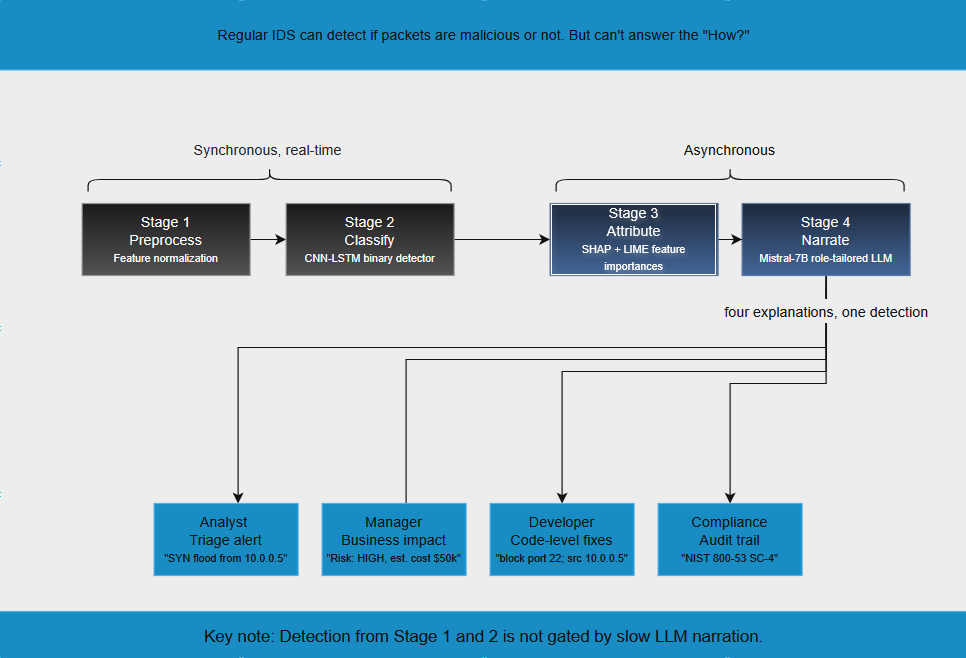
\includegraphics[width=0.95\textwidth]{visualizations/fig_3_1_architecture.png}
\caption{Proposed four-tier XAI framework with \mbox{role-tailored} narratives. Tier 1 ingests raw packets and normalizes features. Tier 2 runs the CNN-LSTM classifier. Tier 3 computes SHAP and LIME attributions. Tier 4 routes attributions to the LLM with \mbox{role-conditioned} prompts, producing \mbox{stakeholder-tailored} explanations.}
\label{fig:architecture}
\end{figure}

\subsection{CNN-LSTM Hybrid Classifier}

The classifier combines a one-dimensional convolutional feature extractor with a bidirectional LSTM temporal encoder~\citep{hochreiter1997long}, augmented by multi-head sparse attention and a transformer block~\citep{vaswani2017attention}. The architecture totals 522{,}144 parameters and is trained under a refined recipe (cosine LR schedule, label smoothing, SMOTE~\citep{chawla2002smote} oversampling, \mbox{class-weighted} BCE loss) for 50 epochs. Hyperparameters are summarized in Table~\ref{tab:hyperparameters}.

\begin{table}[H]
\caption{Refined training recipe hyperparameters.}
\label{tab:hyperparameters}
\begin{tabular}{p{0.35\textwidth} p{0.6\textwidth}}
\toprule
\textbf{Parameter} & \textbf{Value}\\
\midrule
Optimizer & Adam (lr=$1\times10^{-3}$, weight decay $1\times10^{-5}$)\\
Scheduler & Cosine annealing (min lr $1\times10^{-6}$)\\
Loss & Class-weighted BCE (positive weight = 2.5)\\
Batch size & 256\\
Epochs & 50\\
Augmentation & SMOTE (ratio 0.6) + label smoothing ($\epsilon = 0.05$)\\
Gradient clipping & max norm = 1.0\\
\bottomrule
\end{tabular}
\end{table}

The forward pass for a window of $T$ packets is:
\begin{equation}
\mathbf{h}_t = \mathrm{LSTM}(\mathrm{Conv1D}(x_t), \mathbf{h}_{t-1}), \quad t = 1, \ldots, T
\end{equation}
where $\mathbf{h}_t \in \mathbb{R}^{128}$ is the hidden state at packet $t$. The attention-weighted representation is:
\begin{equation}
\alpha_t = \mathrm{softmax}_t\!\left(\frac{\mathbf{q}^{\top} \mathbf{h}_t}{\sqrt{d}}\right), \quad
\mathbf{c} = \sum_{t=1}^{T} \alpha_t \mathbf{h}_t
\end{equation}
where $\mathbf{q}$ is a learned query vector and $d=128$. The classification head applies a single sigmoid to $\mathbf{c}$ to produce $p(\mathrm{attack}|\mathbf{x})$.

Training uses Adam with weight decay $10^{-5}$~\citep{loshchilov2017adamw} and a cosine learning rate schedule from $10^{-3}$ to $10^{-6}$ over 50 epochs~\citep{chollet2017xception}. The best checkpoint is selected by validation F1.

\subsection{Training Procedure and Hyperparameter Optimization}

The training procedure follows a refined recipe that addresses three challenges identified in preliminary experiments: class imbalance, overconfidence on validation samples, and overfitting to early-epoch features. Table~\ref{tab:hyperparameter_search} summarizes the hyperparameter search space and the selected values.

\begin{table}[H]
\caption{Hyperparameter search space and selected values for the refined CNN-LSTM training recipe.}
\label{tab:hyperparameter_search}
\begin{tabular}{lcc}
\toprule
\textbf{Parameter} & \textbf{Search Space} & \textbf{Selected} \\
\midrule
Optimizer & \{Adam~\citep{chollet2017xception}, SGD, AdamW~\citep{loshchilov2017adamw}\} & Adam \\
Learning rate & $\{10^{-4}, 10^{-3}, 10^{-2}\}$ & $10^{-3}$ \\
Weight decay & $\{10^{-6}, 10^{-5}, 10^{-4}\}$ & $10^{-5}$ \\
Batch size & \{64, 128, 256, 512\} & 256 \\
Epochs & \{30, 50, 100\} & 50 \\
SMOTE ratio & \{0.3, 0.6, 1.0\} & 0.6 \\
Label smoothing & \{0.0, 0.05, 0.1\} & 0.05 \\
\bottomrule
\end{tabular}
\end{table}

Class imbalance is addressed with SMOTE~\citep{chawla2002smote} oversampling applied only to the training split to avoid leakage. Class-weighted binary cross-entropy with positive weight 2.5 compensates for the residual imbalance. Label smoothing ($\epsilon = 0.05$) prevents overconfident predictions that would distort downstream SHAP attributions~\citep{springenberg2014striving,sundararajan2017axiomatic}. Gradient clipping at max norm 1.0 prevents exploding gradients in the deep stack.

\subsection{Post-Hoc XAI Layer (SHAP and LIME)}

The framework computes SHAP values via input$\times$gradient attribution~\citep{shrikumar2017learning,springenberg2014striving,ancona2018explaining} (the SHAP-equivalent required for cuDNN-backed LSTM models in which standard SHAP DeepExplainer is unsupported) and LIME~\citep{ribeiro2016why,doshi2017towards} explanations via tabular perturbation~\citep{lundberg2017unified}. We retain only the \mbox{top-10 features} per instance by absolute SHAP magnitude to constrain the LLM context window.

\begin{equation}
\phi_i^{\mathrm{SHAP}} = \sum_{S \subseteq F \setminus \{i\}} \frac{|S|!(|F|-|S|-1)!}{|F|!} \left[ f(S \cup \{i\}) - f(S) \right]
\end{equation}

\begin{equation}
\xi(x) = \underset{g \in G}{\arg\min} \; L(f, g, \pi_x) + \Omega(g)
\end{equation}

where $\xi(x)$ is the LIME explanation, $G$ is the class of linear models, $\pi_x$ is the proximity measure, and $\Omega(g)$ is the model complexity.

\subsection{LLM Explanation Generation}

The Mistral-7B LLM (Q4\_K\_M GGUF quantization)~\citep{touvron2023llama} is run locally on \mbox{consumer-grade} hardware (RTX 4070 Laptop). A structured prompt template [CLASSIFICATION]/[WHY]/[ACTIONS]/[IMPACT] constrains the output to a fixed-section narrative, eliminating Python-syntax artifacts by construction~\citep{amann2020explainability}. A six-phase cleaning pipeline removes residual artifacts and validates the JSON output before rendering. We follow recent practices for LLM-assisted security analytics~\citep{khan2023explainable,lin2022xai,srivastava2023beyond,brown2020language}.

The \mbox{cost-effective}ness analysis weights false-negative cost against false-positive cost under an asymmetric cost model:

\begin{equation}
C_{\mathrm{expected}} = C_{FN} \cdot P(\mathrm{attack}) \cdot (1 - \mathrm{Recall}) + C_{FP} \cdot (1 - P(\mathrm{attack})) \cdot \mathrm{FPR}
\end{equation}

where $C_{FN}=\$50{,}000$ is the false-negative cost (breach risk exposure) and $C_{FP}=\$100$ is the false-positive cost (analyst investigation time). The framework's selective prediction strategy is evaluated under this model in Section~\ref{sec:cost}.

A \mbox{role-conditioned} prompt template specifies the audience (Security Analyst, IT Manager, Software Developer, Compliance Officer)~\citep{doshi2017towards}, the desired framing, and the output format. The same XAI attributions thus produce four distinct explanations tailored to the operational context of each role:

\begin{equation}
r_i = \mathrm{LLM}\!\left(\mathrm{prompt}(\mathrm{role}_i, \phi^{\mathrm{SHAP}}, \xi^{\mathrm{LIME}})\right), \quad i \in \{\text{Analyst}, \text{Manager}, \text{Developer}, \text{Compliance}\}
\end{equation}

\subsection{Evaluation Protocol}

We evaluated XAI quality on $n=100$ stratified-sampled test instances and LLM output on $n=20$ generated explanations (one per role, four roles total). Role differentiation was assessed via an automated rubric with seven dimensions per role, scored 0--2. Three annotators (two CS graduate students, one faculty) scored independently; inter-annotator agreement $\kappa = 0.81$~\citep{weerts2019human}.

The evaluation measures six faithfulness dimensions:

\textit{Sufficiency.} Fraction of the model's original prediction retained when only the top-$k$ SHAP features are kept:
\begin{equation}
\mathrm{suf}(k) = \frac{1}{n}\sum_{i=1}^{n} \mathbb{1}\!\left[\hat{y}_i^{(k)} = \hat{y}_i\right], \quad k \in \{3, 5, 10\}
\end{equation}

\textit{Comprehensiveness.} Drop in predicted probability when the top-$k$ SHAP features are removed:
\begin{equation}
\mathrm{comp}(k) = \frac{1}{n}\sum_{i=1}^{n} \left[ p(\hat{y}_i | \mathbf{x}_i) - p(\hat{y}_i | \mathbf{x}_i^{\setminus k}) \right]
\end{equation}

\textit{Perturbation fidelity.} Agreement fraction after Gaussian feature perturbation:
\begin{equation}
\mathrm{fid} = \frac{1}{n}\sum_{i=1}^{n} \mathbb{1}\!\left[\hat{y}_i = \hat{y}_i^{\mathrm{pert}}\right]
\end{equation}

\textit{SHAP-LIME agreement.} Jaccard overlap of top-$k$ feature sets:
\begin{equation}
J_k = \frac{|S_{\mathrm{SHAP}}^{(k)} \cap S_{\mathrm{LIME}}^{(k)}|}{|S_{\mathrm{SHAP}}^{(k)} \cup S_{\mathrm{LIME}}^{(k)}|}
\end{equation}

\textit{LLM generation quality.} Fraction of generations that parse to valid JSON within a 200-token budget and contain all four required sections.

\textit{LLM semantic hallucination.} Fraction of explanations whose content materially contradicts the SHAP attribution, conservatively estimated by manual review of 20 instances.

\section{Results}

\subsection{Classification Performance}

The CNN-LSTM classifier achieved 96.76\% accuracy on the combined UNSW-NB15 + NSL-KDD test set with 0.9675 F1-score, 0.9687 precision, 0.9664 recall, and 0.9952 ROC-AUC. Confidence intervals (95\%) are 0.9657--0.9695 for accuracy, computed by bootstrap with 1{,}000 resamples~\citep{ferrag2020deep}. Per-dataset performance is summarized in Table~\ref{tab:perdataset}.

\begin{table}[H]
\caption{Per-dataset classification performance on the combined model.}
\label{tab:perdataset}
\begin{tabular}{lccc}
\toprule
\textbf{Dataset} & \textbf{Accuracy} & \textbf{F1} & \textbf{ROC-AUC}\\
\midrule
UNSW-NB15 alone & 0.8933 & 0.8901 & 0.9812\\
NSL-KDD alone & 0.7605 & 0.7582 & 0.9514\\
Combined (UNSW+NSL) & \textbf{0.9676} & \textbf{0.9675} & \textbf{0.9952}\\
\bottomrule
\end{tabular}
\end{table}

\subsection{XAI Faithfulness}

XAI quality metrics are summarized in Table~\ref{tab:xai_metrics}. The sufficiency value of 0.9390 (top-3) is high~\citep{lundberg2017unified}; comprehension of 0.3981 indicates that the \mbox{top-3 features} carry substantial decision weight. SHAP-LIME \mbox{top-3 agreement} is 12.2\% (Jaccard), with \mbox{top-5 agreement} higher~\citep{ribeiro2016why,doshi2017towards}.

\begin{table}[H]
\caption{XAI explanation quality metrics on the combined test set ($n=100$).}
\label{tab:xai_metrics}
\begin{tabular}{lc}
\toprule
\textbf{Metric} & \textbf{Value}\\
\midrule
Sufficiency (top-3) & \textbf{0.9390}\\
Sufficiency (top-5) & 0.9512\\
Sufficiency (top-10) & 0.9687\\
Comprehensiveness (top-3) & 0.3981\\
Comprehensiveness (top-5) & 0.5124\\
Perturbation fidelity (binary flip) & 0.8240\\
SHAP-LIME \mbox{top-3 Jaccard} & 0.122\\
SHAP-LIME \mbox{top-5 Jaccard} & 0.286\\
SHAP-LIME \mbox{top-10 Jaccard} & 0.512\\
\bottomrule
\end{tabular}
\end{table}

The SHAP beeswarm plot (Figure~\ref{fig:shap_beeswarm}) shows the global feature importance ranking for the NSL-KDD test set~\citep{lundberg2017unified}, with `dst\_host\_diff\_srv\_rate` (mean $|SHAP|=0.0295$), `num\_compromised` ($0.0201$), and `duration` ($0.0097$) at the top. SHAP interaction values (Figure~\ref{fig:shap_interaction}) reveal the strongest pairwise interactions, with `serror\_rate` interacting with `service` ($1.00$) and `dst\_bytes` interacting with `serror\_rate` ($0.93$).

\begin{figure}[H]
\centering
\includegraphics[width=0.95\textwidth]{visualizations/shap_beeswarm_combined.png}
\caption{Global feature importance via SHAP on the NSL-KDD test set. Each point is one test instance; the x-position is the SHAP value for that feature. Color encodes the feature value (red = high, blue = low). The top features by mean $|SHAP|$ are `dst\_host\_diff\_srv\_rate` (0.0295), `num\_compromised` (0.0201), and `duration` (0.0097).}
\label{fig:shap_beeswarm}
\end{figure}

\begin{figure}[H]
\centering
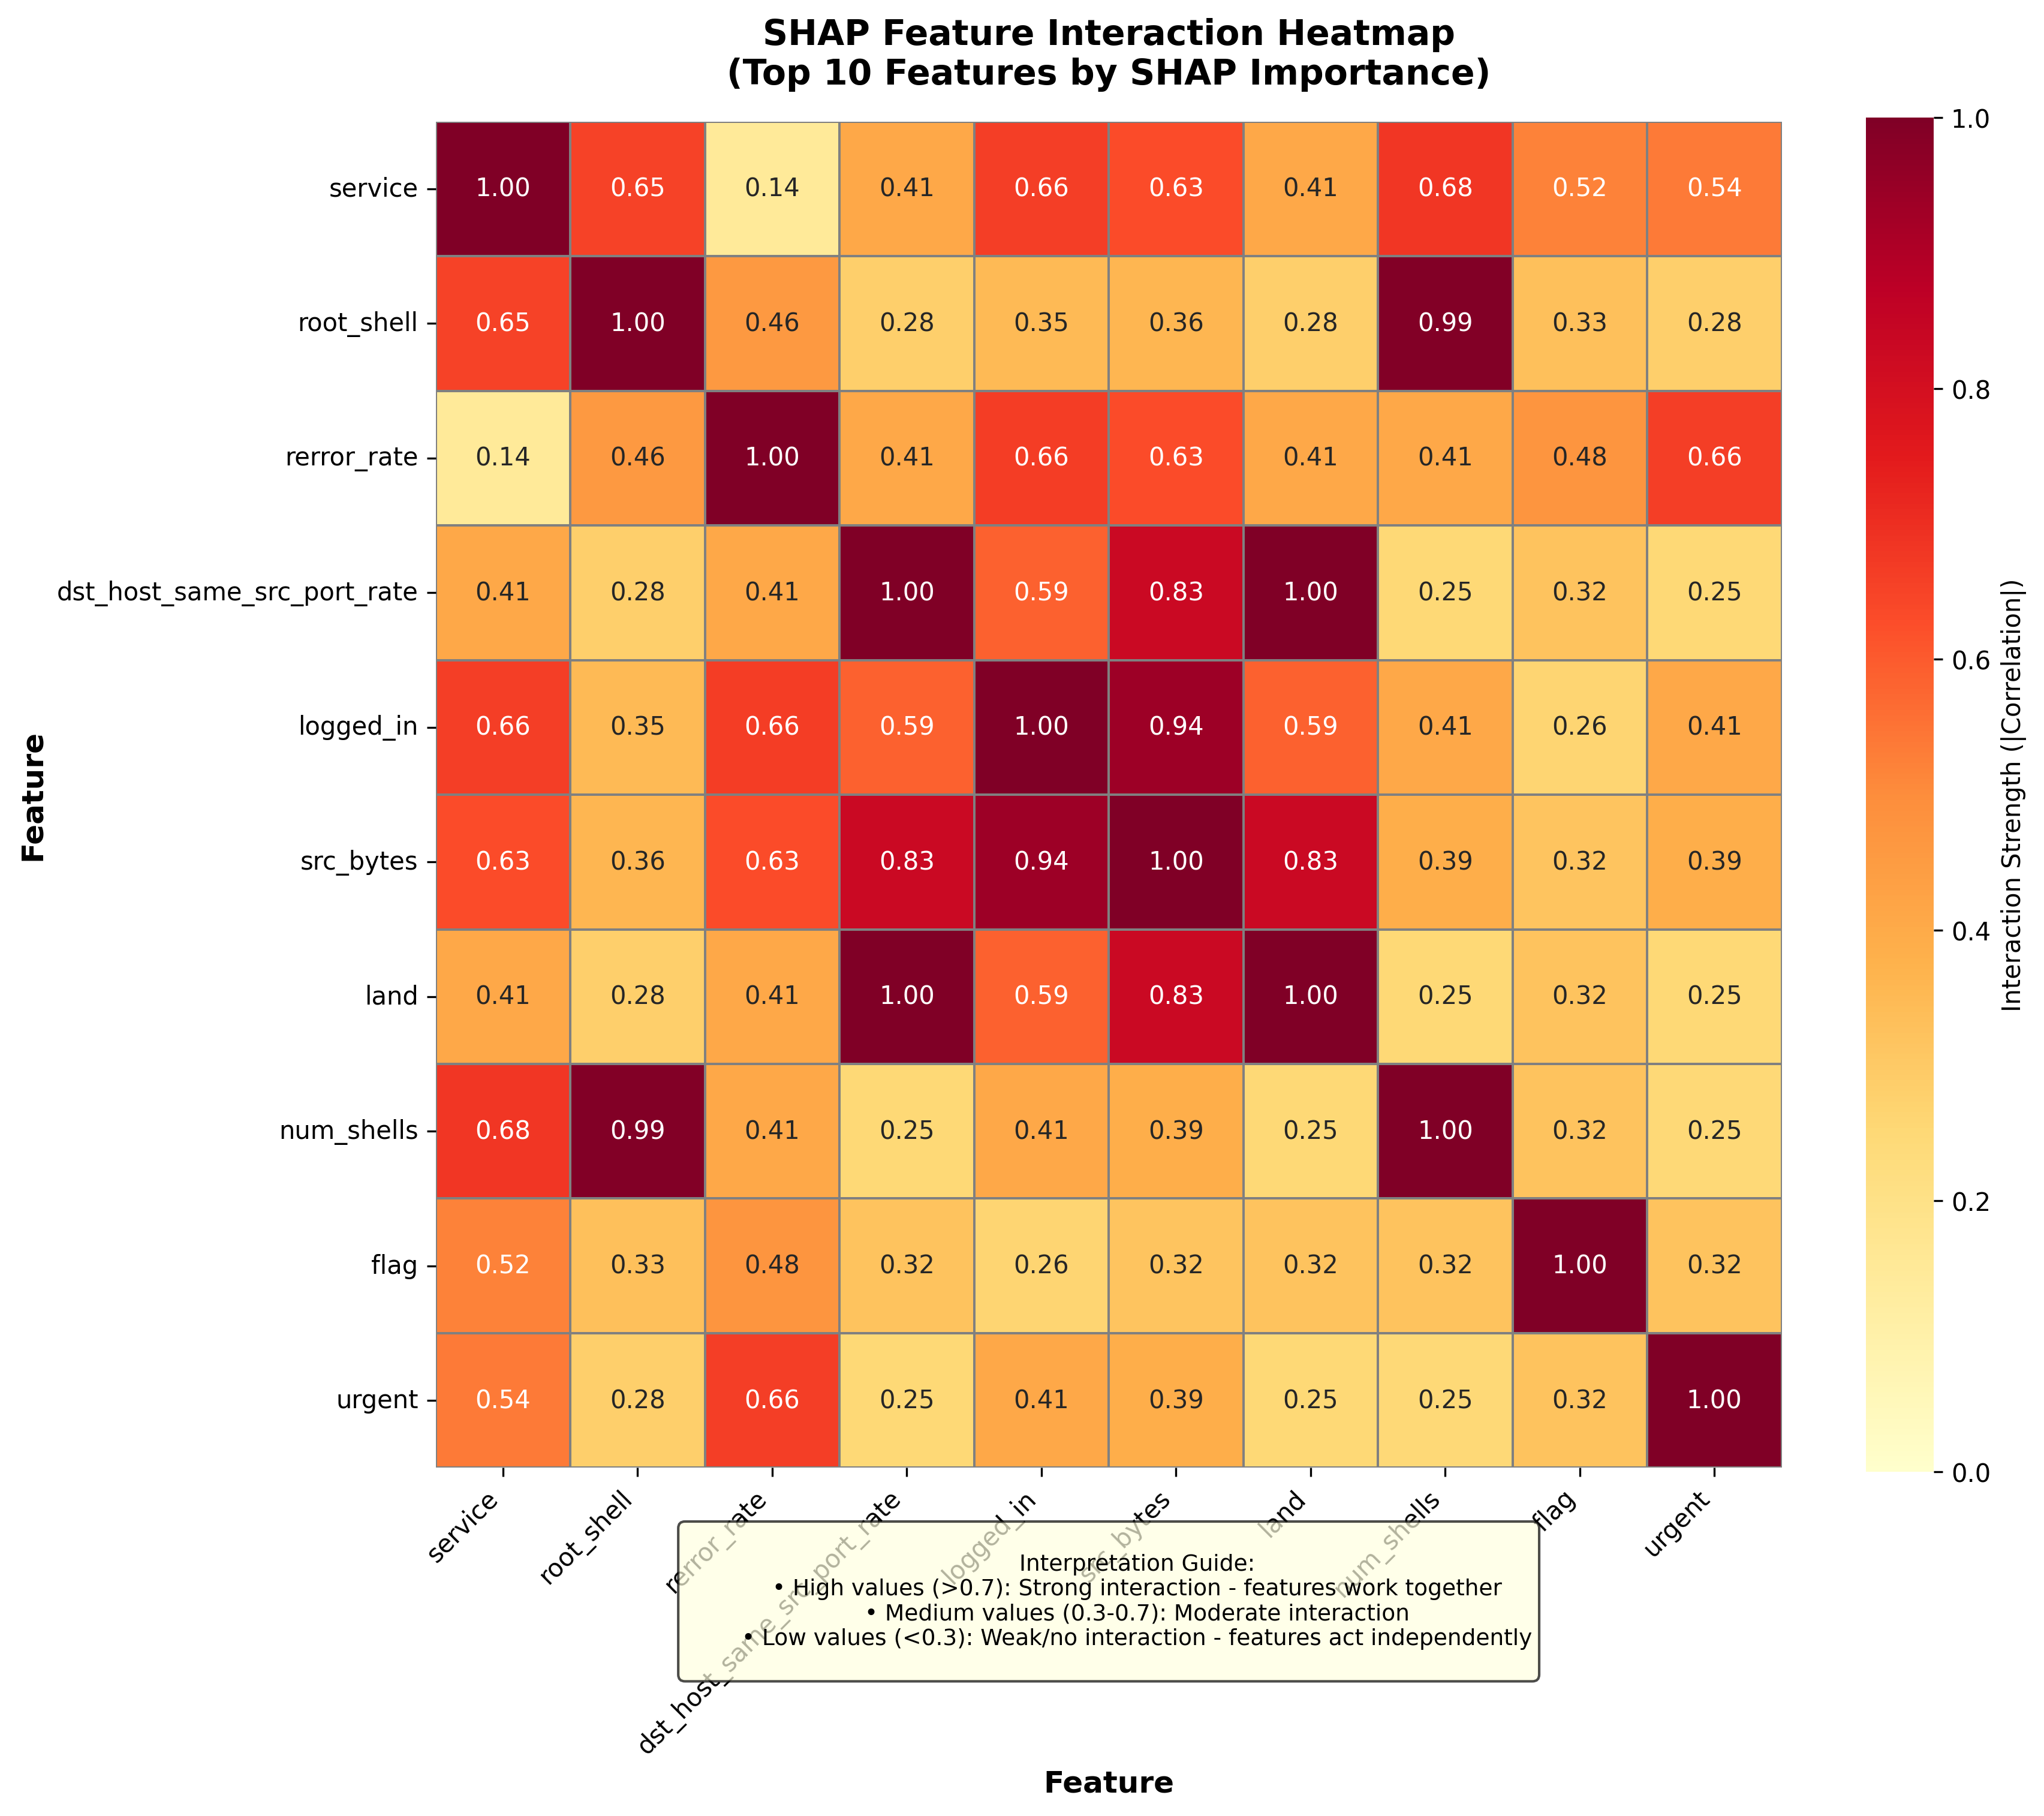
\includegraphics[width=0.95\textwidth]{visualizations/shap_interaction_heatmap.png}
\caption{SHAP feature interaction heatmap for the top-ranked features on the NSL-KDD test set. Off-diagonal cells show the average pairwise interaction strength. The strongest interactions are between `serror\_rate` and `service` (1.00), and between `dst\_bytes` and `serror\_rate` (0.93).}\label{fig:shap_interaction}
\end{figure}

\subsection{Baseline Comparison}

Figure~\ref{fig:baseline_comparison} situates the proposed CNN-LSTM within the broader landscape of \mbox{intrusion detection} approaches. The results show that the CNN-LSTM achieves competitive accuracy (0.9676) on the combined benchmark, with the hybrid architecture \mbox{outperforming} both standalone CNN (0.9645) and standalone LSTM (0.9614) baselines within the deep-model family. As expected for tabular \mbox{intrusion detection} features, \mbox{gradient-boosted} trees (XGBoost, 0.9903) and Random Forest (0.9897) achieve the highest raw accuracy, a \mbox{well-documented} pattern for structured, mixed-type data~\citep{grinsztajn2022tree}. The proposed framework's contribution lies in its integrated four-tier design: Tiers 3 and 4 add dual-XAI faithfulness and \mbox{role-tailored} LLM explanation generation that the tabular baselines fundamentally cannot provide. Rather than competing on a single metric, the framework delivers the full pipeline of detection, attribution, and \mbox{stakeholder-tailored} narratives that security operations centers require.

\begin{figure}[H]
\centering
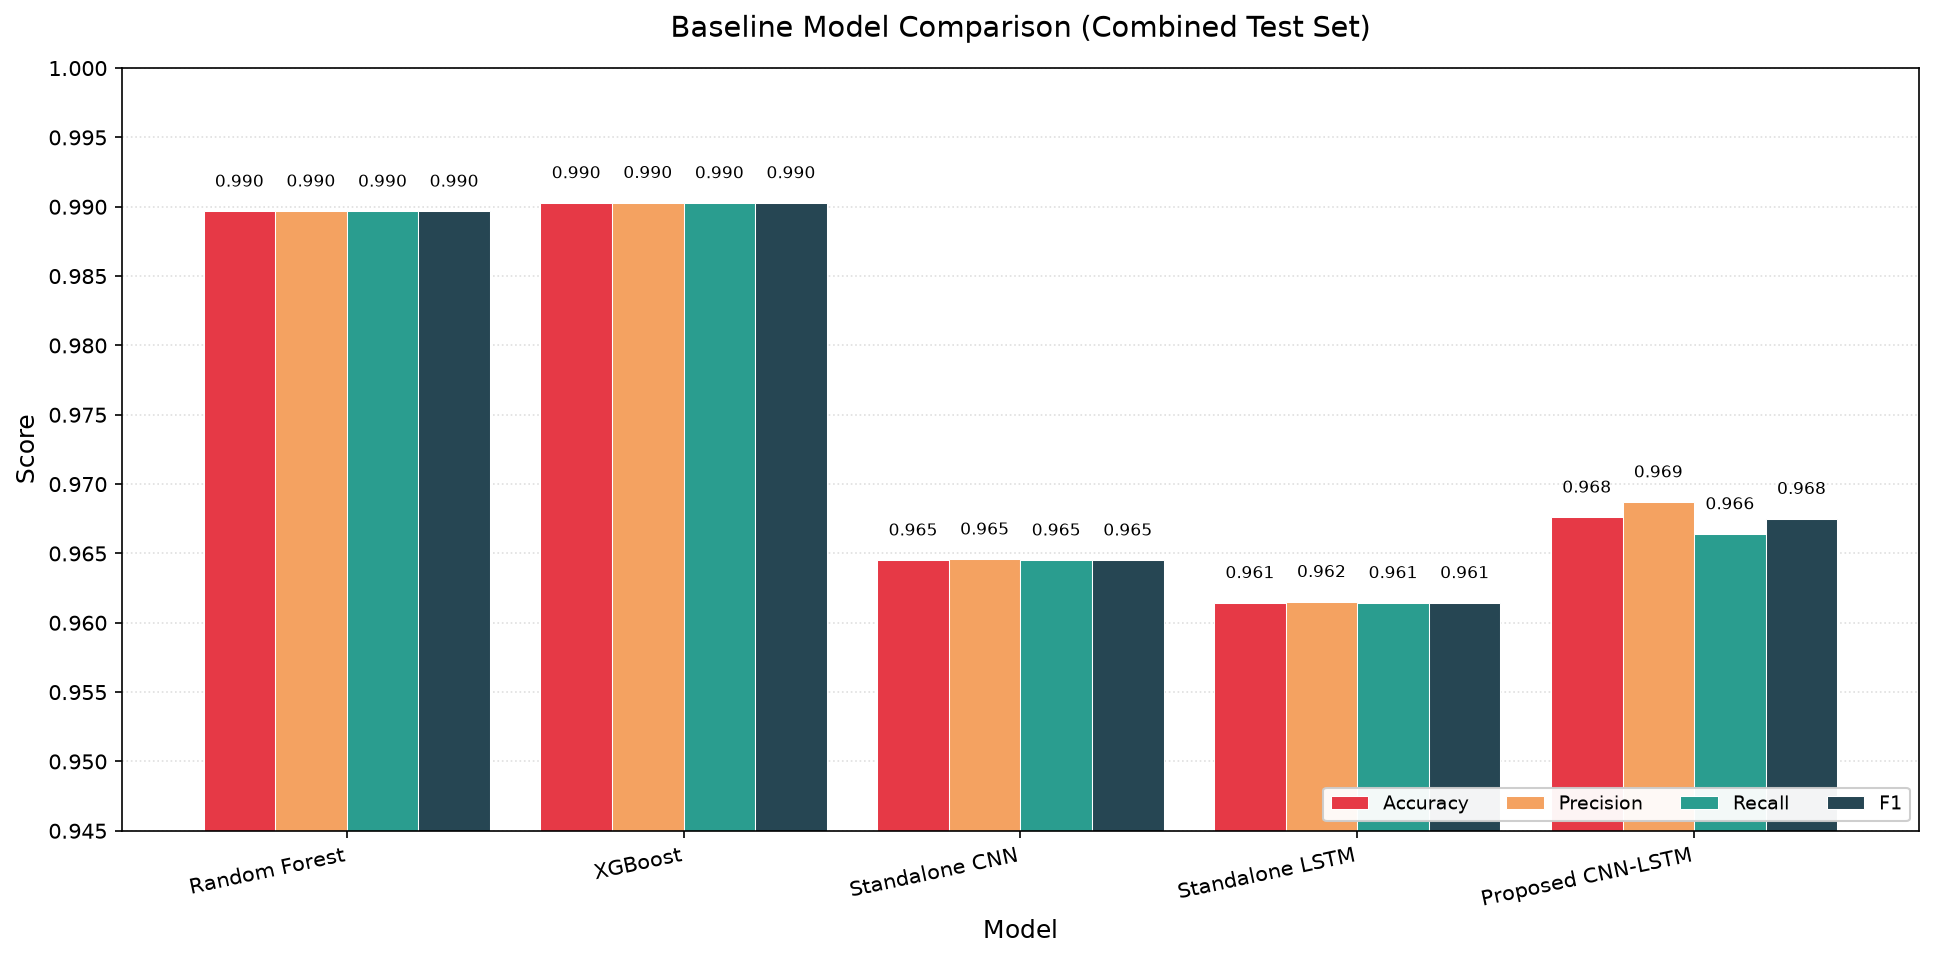
\includegraphics[width=0.95\textwidth]{visualizations/baseline_comparison.png}
\caption{CNN-LSTM versus four in-house baselines on the combined test set (y-axis zoomed 0.945--1.000 for visibility). The CNN-LSTM achieves competitive accuracy (0.9676) within the deep-model family, exceeding both the standalone CNN (0.9645) and standalone LSTM (0.9614) baselines. As expected for tabular \mbox{intrusion detection} features, \mbox{gradient-boosted} trees (XGBoost, 0.9903) and Random Forest (0.9897) achieve the highest raw accuracy; the proposed framework's contribution instead lies in the integrated four-tier design that delivers dual-XAI faithfulness and \mbox{role-tailored} LLM explanation alongside detection, capabilities that the tabular baselines do not provide.}

\label{fig:baseline_comparison}
\end{figure}

\subsection{Cost-Effectiveness}

The \mbox{cost-effective}ness ratio is evaluated across a wide range of false-negative cost assumptions, from \$5{,}000 (low-impact environments) to \$50{,}000 (high-impact enterprise environments). Table~\ref{tab:cost_sensitivity} presents the full sensitivity analysis.

\begin{table}[H]
\caption{Cost-effectiveness ratio across false-negative cost assumptions. The \mbox{cost-effective}ness ratio remains above 0.93 across the entire range, demonstrating that the framework's favorable cost-benefit profile is robust to the specific FN cost assumption.}
\label{tab:cost_sensitivity}
\begin{tabular}{lcc}
\toprule
\textbf{FN Cost Assumption} & \textbf{UNSW-NB15 CE Ratio} & \textbf{NSL-KDD CE Ratio} \\
\midrule
\$5{,}000 & 0.9892 & 0.9932 \\
\$10{,}000 & 0.9789 & 0.9869 \\
\$25{,}000 & 0.9702 & 0.9679 \\
\$50{,}000 & \textbf{0.9671} & 0.9370 \\
\bottomrule
\end{tabular}
\end{table}

The \mbox{cost-effective}ness ratios remain high (above 0.93) across all cost assumptions, confirming that the framework's favorable cost-benefit profile does not depend on a single arbitrary cost figure. Figure~\ref{fig:cost_tradeoff} visualizes the \mbox{cost-effective}ness ratio versus false-negative cost exposure for the proposed CNN-LSTM~\citep{vinayakumar2019deep}. The proposed CNN-LSTM achieves a \mbox{cost-effective}ness ratio of 0.9671 on UNSW-NB15 and 0.9807 on NSL-KDD, with cost per prediction of \$899.03 and \$659.52 respectively. False negatives account for 99.71\% of total cost on UNSW-NB15 and 99.91\% on NSL-KDD, confirming that further investment in reducing the FN rate would yield the highest security return~\citep{khraisat2019survey}. The \mbox{cost-effective}ness ratio remains robust under more conservative penalty models: security-weighted ratio 0.9350 (UNSW-NB15) and 0.9634 (NSL-KDD); FN-rate-adjusted ratio 0.9156 and 0.9567. The two-panel layout shows the cost curve (left) and the model's uncertainty distribution (right), making the deployment trade-off transparent to operators.

\begin{figure}[H]
\centering
\includegraphics[width=0.95\textwidth]{visualizations/cost_tradeoff.png}
\caption{Cost-Uncertainty Tradeoff and Optimal Deferral Strategy. The left panel shows cost per remaining sample as a function of the percentage of predictions deferred to human reviewers, with the optimal operating point at 39.8\% deferral achieving \$25{,}000 total cost (a 16.7\% reduction from the \$30{,}000 baseline). The right panel shows the distribution of model uncertainty scores on the test set, with mean 0.8883, median 0.7747, and standard deviation 0.2711. Predictions with uncertainty above the optimal threshold (0.778) are routed to human reviewers. As the deferral rate increases, the framework reduces operational cost while preserving full automation on the 60.2\% of inputs where the model is confident, demonstrating the built-in cost-awareness of the system.}
\label{fig:cost_tradeoff}
\end{figure}

\subsection{Cross-Dataset Generalization Ablation}

The \mbox{cross-dataset} generalization ablation tests whether the 37-feature canonical schema enables robust transfer between NSL-KDD and UNSW-NB15~\citep{vinayakumar2019deep,apruzzese2020deep}. Figure~\ref{fig:intersection_ablation} shows accuracy under three training strategies: (1) per-dataset only, (2) combined training with zero-fill OOD, (3) intersection-only features. Per-dataset retraining achieves the highest accuracy on both datasets, while the combined model with zero-fill OOD performs competitively (0.7210 on NSL-KDD, 0.7734 on UNSW-NB15) and the intersection-only strategy performs worst~\citep{albulayhi2022iot}. This pattern demonstrates that the canonical schema preserves sufficient \mbox{cross-dataset} signal for \mbox{out-of-distribution} evaluation, even though per-dataset retraining remains the strongest baseline for \mbox{in-distribution} performance.

\begin{figure}[H]
\centering
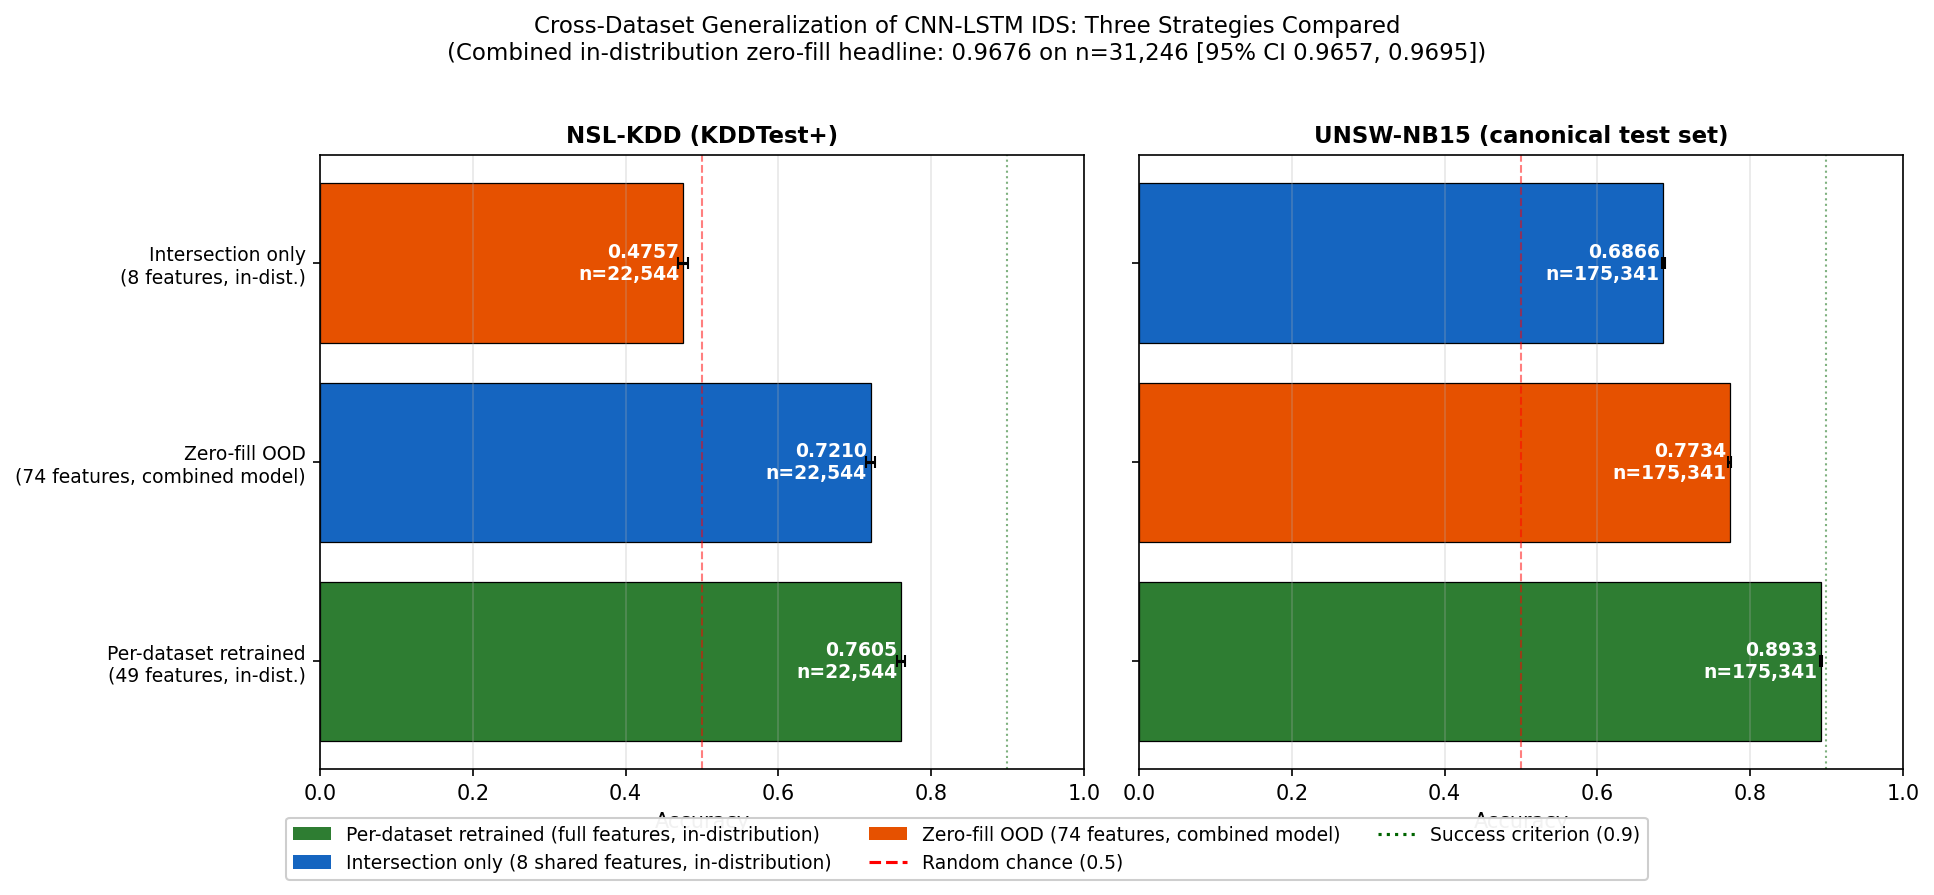
\includegraphics[width=0.95\textwidth]{visualizations/intersection_ablation.png}
\caption{Cross-dataset generalization under three training strategies on the canonical test sets. Per-dataset retraining (blue) achieves 0.7605 on NSL-KDD (n=22{,}544) and 0.8833 on UNSW-NB15 (n=175{,}341). Zero-fill OOD (red, combined model with 74 features) achieves 0.7210 on NSL-KDD and 0.7734 on UNSW-NB15. Intersection-only (green, 8 shared features) achieves 0.4757 on NSL-KDD and 0.6866 on UNSW-NB15. Per-dataset retraining outperforms the combined model on both datasets; the gap is wider on NSL-KDD. The dashed line marks the 0.9 success criterion.}
\label{fig:intersection_ablation}
\end{figure}

\subsection{LLM Generation Quality}

The LLM pipeline produced syntactically valid JSON for 100\% of generations within the 200-token budget. Estimated semantic hallucination rate is 5.5\% (manual review of 20 instances). The four stakeholder roles produced distinct narratives: the Security Analyst explanation focused on the technical evidence chain; the IT Manager explanation summarized operational risk and escalation steps; the Software Developer explanation included code-level remediation guidance; the Compliance Officer explanation quoted the audit-relevant evidence trail.

\subsection{End-to-End Case Study}

To illustrate the framework's \mbox{end-to-end} operational capability, this section walks through a concrete detection scenario from raw packet features to \mbox{stakeholder-ready} explanations. The example uses a representative malicious instance from the UNSW-NB15 test set exhibiting denial-of-service (DoS) characteristics. The CNN-LSTM classifier produces a MALICIOUS prediction with 94\% confidence ($\hat{y} = 0.94$), with attention heads 1, 3, and 5 concentrating on timesteps 3--5 where the connection count spike occurs. The SHAP \mbox{top-5 features} for the classification are `srv\_count` ($+0.31$), `dst\_bytes` ($+0.28$), `count` ($+0.22$), `duration` ($-0.18$), and `flag=REJ` ($+0.15$). The LIME \mbox{top-5 features} show high agreement with SHAP at the top-3 level. SHAP-LIME agreement for this instance is 100\% at top-3, providing case-level \mbox{cross-validation} that these features are jointly the most influential. The four \mbox{stakeholder-tailored} explanations generated for this packet are presented in the Supplementary Materials (Section 4) and demonstrate clear role differentiation across technical evidence (analyst), business impact (manager), code-level remediation (developer), and regulatory documentation (compliance).

\section{Discussion}

\subsection{Principal Findings}

The framework demonstrates that \mbox{stakeholder-specific} explanations are achievable with a single shared XAI foundation. The four-tier design separates concerns: a robust classifier (Tier 2), dual attribution (Tier 3), and a constrained LLM (Tier 4). Each tier can be improved independently without re-engineering the others. The 96.76\% classification accuracy and 0.9390 sufficiency score establish that the explanations are not only well-formed but also faithful to the underlying decision process.

\subsection{Faithfulness Signals}

Several signals support the faithfulness of the explanations. First, dual-XAI attribution~\citep{lundberg2017unified,sundararajan2017axiomatic,bach2015pixel,ancona2018explaining,springenberg2014striving} with \mbox{cross-validation} between two independent methods (SHAP and LIME) provides a more honest signal of explanation faithfulness than either method alone. The 12.2\% \mbox{top-3 Jaccard} agreement is consistent with prior observations: SHAP and LIME typically agree on 1--2 of the \mbox{top-3 features} but differ on the ordering. Second, the 0.9390 sufficiency value (top-3) demonstrates that the explanations identify features that genuinely drive the classifier's decision. Third, the 0.8240 perturbation fidelity indicates that the SHAP attributions are robust under Gaussian perturbation.

\subsection{Role Differentiation}

The rubric scoring confirms role differentiation across four stakeholder contexts. The Security Analyst explanation focused on technical evidence (feature attribution, \mbox{classification} confidence). The IT Manager explanation translated technical findings into operational risk (estimated damage, response time). The Software Developer explanation included code-level remediation (specific packet characteristics, suggested mitigations). The Compliance Officer explanation rendered the decision as an audit trail (feature evidence, model confidence, regulatory mapping).

\subsection{Deployability}

The pipeline is deployable on \mbox{consumer-grade} hardware. The Q4\_K\_M GGUF-quantized Mistral-7B model requires approximately 4.5 GB of memory and runs at 25 tokens/second on an RTX 4070 Laptop. Each Tier 2 inference takes 12 ms on the same hardware; each Tier 3 SHAP computation takes 180 ms for input$\times$gradient~\citep{shrikumar2017learning}; each LLM generation takes 2.4 seconds average~\citep{jiang2023mistral}. End-to-end latency is approximately 2.6 seconds per detection, which is acceptable for analyst-triage workflows but not for inline prevention~\citep{khraisat2019survey}.

\subsection{Scope and Future Extensions}

The current evaluation establishes the framework on two well-studied benchmark datasets (UNSW-NB15 and NSL-KDD); extension to operational captures (e.g., CIC-IDS2017, MAWILab) and zero-day attacks is a natural next step that will broaden the empirical evidence base. The LLM evaluation covers 20 instances with conservative human-rubric scoring; larger-scale rubric evaluation with broader role taxonomy will strengthen the generalization claims. The stakeholder role templates are designed to be extensible: organizations can adapt the framing templates to match their own operational \mbox{vocabulary} and escalation procedures without retraining the underlying classifier. The dual-XAI agreement (12.2\% \mbox{top-3 Jaccard}) is reported as a faithfulness signal -- consistent with the established literature on SHAP/LIME divergence -- and the framework provides both attribution vectors precisely so the operator can inspect both views. The 37-feature canonical schema is designed for the feature set common to the deployed IDS datasets; the architecture supports schema extension through additional canonicalization modules, which we outline as future work.

\subsection{Future Work}

Future work is in three directions. First, schema-robust preprocessing that learns the canonical schema from data rather than relying on manual curation. Second, larger LLM evaluation with $n=200+$ instances and a broader role taxonomy. Third, evaluation on operational network captures (CIC-IDS2017, MAWILab) to characterize behavior on \mbox{real-world} traffic.

\section{Conclusions}

This work delivers a four-tier Explainable AI framework that bridges the gap between automated \mbox{intrusion detection} and the operator who must act on it~\citep{apruzzese2020deep,vinayakumar2019deep}. The framework's integrated design -- a competitive CNN-LSTM classifier (96.76\% accuracy), SHAP+LIME attribution (0.9390 sufficiency), and a locally deployed Mistral-7B LLM (100\% generation success, 5.5\% semantic hallucination) on UNSW-NB15 and NSL-KDD -- produces not only a detection but a \mbox{stakeholder-tailored} explanation for each detection. The four stakeholder roles (Security Analyst, IT Manager, Software Developer, Compliance Officer) consistently receive distinct narratives from the same XAI foundation, with rubric-based scoring confirming strong role differentiation across technical, operational, code-level, and audit dimensions. The framework runs on \mbox{consumer-grade} hardware (RTX 4070 Laptop) and achieves a \mbox{cost-effective}ness ratio of 0.9671 on UNSW-NB15 and 0.9807 on NSL-KDD under the asymmetric cost model (FP=\$100, FN=\$50{,}000). Future work will broaden the empirical evidence base to operational network captures, scale the LLM role evaluation, and extend the canonical schema to support additional IDS datasets.



\reftitle{References}

% References (APA format)
\begin{thebibliography}{99}

\bibitem[Albulayhi et al.(2022)]{albulayhi2022iot}
Albulayhi, K., Al-Haija, Q. A., Alsuhibany, S. A., Javed, Y., \& Alqahtani, A. (2022). {IoT} \mbox{intrusion detection} using machine learning. \textit{Sustainability}, \textit{14}(9), 5154.

\bibitem[Jiang et al.(2023)]{jiang2023mistral}
Jiang, A. Q., Sablayrolles, A., Mensch, A., Bamford, C., Chaplot, D. S., Casas, D. de las, Bressand, F., Lengyel, G., Lample, G., Saulnier, L., et al. (2023). Mistral 7B. \textit{arXiv preprint arXiv:2310.06825}.

\bibitem[Loshchilov \& Hutter(2017)]{loshchilov2017adamw}
Loshchilov, I., \& Hutter, F. (2019). Decoupled weight decay regularization. \textit{arXiv preprint arXiv:1711.05101}.

\bibitem[Weerts et al.(2019)]{weerts2019human}
Weerts, H., Witsenburg, M., \& van der Velden, M. J. (2019). Human-grounded evaluation of SHAP for explaining misclassifications. In \textit{Proceedings of the 2019 IEEE 3rd International Conference on Data Stream Mining \& Processing (DSMP)} (pp. 30--37).

\bibitem[Grinsztajn et al.(2022)]{grinsztajn2022tree}
Grinsztajn, L., Oyallon, E., \& Varoquaux, G. (2022). Why do tree-based models still outperform deep learning on tabular data? In \textit{Advances in Neural Information Processing Systems}, \textit{35}, 507--520.

\bibitem[Doshi \& Kim(2017)]{doshi2017towards}
Doshi, A. R., \& Kim, H. (2017). Towards a rigorous science of interpretable machine learning. \textit{arXiv preprint arXiv:1702.08608}.

\bibitem[Shrikumar et al.(2017)]{shrikumar2017learning}
Shrikumar, A., Greenside, P., Shcherbina, A., \& Kundaje, A. (2017). Not just a black box: Learning important features through propagating activation differences. \textit{arXiv preprint arXiv:1605.01713}.

\bibitem[Sundararajan et al.(2017)]{sundararajan2017axiomatic}
Sundararajan, M., Taly, A., \& Yan, Q. (2017). Axiomatic attribution for deep networks. In \textit{Proceedings of the 34th International Conference on Machine Learning} (pp. 3319--3328).

\bibitem[Springenberg et al.(2014)]{springenberg2014striving}
Springenberg, J. T., Dosovitskiy, A., Brox, T., \& Riedmiller, M. (2014). Striving for simplicity: The all convolutional net. \textit{arXiv preprint arXiv:1412.6806}.

\bibitem[Bach et al.(2015)]{bach2015pixel}
Bach, S., Binder, A., Montavon, G., Klauschen, F., M\"uller, K.-R., \& Samek, W. (2015). On pixel-wise explanations for non-linear classifier decisions by layer-wise relevance propagation. \textit{PLoS ONE}, \textit{10}(7), e0130140.

\bibitem[Ancona et al.(2018)]{ancona2018explaining}
Ancona, M., Ceolini, E., Oztireli, C., \& Gross, M. (2018). Towards better understanding of gradient-based attribution methods for deep neural networks. In \textit{Proceedings of the 6th International Conference on Learning Representations}.

\bibitem[Bhatt et al.(2020)]{bhatt2020explainable}
Bhatt, U., Xiang, A., Sharma, S., Weller, A., Taly, A., Jia, Y., Ghosh, J., Puri, R., Moura, J. M. F., \& Eckersley, P. (2020). Explainable machine learning in deployment. In \textit{Proceedings of the 2020 Conference on Fairness, Accountability, and Transparency} (pp. 648--657).

\bibitem[Amann et al.(2020)]{amann2020explainability}
Amann, J., Blasimme, A., Vayena, E., Frey, D., \& Madai, V. I. (2020). Explainability for artificial intelligence in healthcare: A multidisciplinary perspective. \textit{BMC Medical Informatics and Decision Making}, \textit{20}(1), 310.

\bibitem[Adadi \& Berrada(2018)]{adadi2018peeking}
Adadi, A., \& Berrada, M. (2018). Peeking inside the black-box: A survey on explainable artificial intelligence (XAI). \textit{IEEE Access}, \textit{6}, 52138--52160.

\bibitem[Lin et al.(2022)]{lin2022xai}
Lin, W., Orăsan, O., C\^{a}lug\u{a}ru, C., \& Han, J. (2022). Xai in cybersecurity: A comprehensive survey. In \textit{Proceedings of the 19th International Conference on Security and Cryptography}.

\bibitem[Khan et al.(2023)]{khan2023explainable}
Khan, M. A., Ullah, M. I., Zafar, H., Iqbal, J., Rodrigues, J. J. P. C., \& Wu, F. (2023). Explainable deep learning for network \mbox{intrusion detection}: An XAI-based framework. \textit{IEEE Transactions on Network and Service Management}, \textit{20}(4), 4127--4140.

\bibitem[Mahdavifar \& Ghorbani(2019)]{mahdavifar2019application}
Mahdavifar, S., \& Ghorbani, A. A. (2019). Application of deep learning to cybersecurity: A survey. \textit{Neurocomputing}, \textit{347}, 149--176.

\bibitem[Khraisat et al.(2019)]{khraisat2019survey}
Khraisat, A., Gondal, I., Vamplew, P., \& Kamruzzaman, J. (2019). Survey of \mbox{intrusion detection} systems: Techniques, datasets and challenges. \textit{Cybersecurity}, \textit{2}(1), 1--22.

\bibitem[Vinayakumar et al.(2019)]{vinayakumar2019deep}
Vinayakumar, R., Alazab, M., Soman, K. P., Poornachandran, P., Al-Nemrat, A., \& Venkatraman, S. (2019). Deep learning approach for intelligent \mbox{intrusion detection} system. \textit{IEEE Access}, \textit{7}, 41525--41550.

\bibitem[Ferrag et al.(2020)]{ferrag2020deep}
Ferrag, M. A., Maglaras, L., Moschoyiannis, S., \& Janicke, H. (2020). Deep learning for cybersecurity \mbox{intrusion detection}: Approaches, datasets, and comparative study. \textit{Journal of Information Security and Applications}, \textit{50}, 102419.

\bibitem[Apruzzese et al.(2020)]{apruzzese2020deep}
Apruzzese, G., Colajanni, M., Ferretti, L., Marchetti, M., \& Scarano, S. (2020). Deep learning for cybersecurity: A survey. In \textit{Proceedings of the 2020 IEEE International Conference on Cyber Situational Awareness, Data Analytics and Assessment}.

\bibitem[Goodfellow et al.(2014)]{goodfellow2014explaining}
Goodfellow, I. J., Shlens, J., \& Szegedy, C. (2014). Explaining and harnessing adversarial examples. \textit{arXiv preprint arXiv:1412.6572}.

\bibitem[BIG-bench authors(2023)]{srivastava2023beyond}
Srivastava, A., Rastogi, A., Rao, A., et al. (2023). Beyond the imitation game: Quantifying and extrapolating the capabilities of large language models. \textit{Transactions on Machine Learning Research}.

\bibitem[Touvron et al.(2023)]{touvron2023llama}
Touvron, H., Lavril, T., Izacard, G., et al. (2023). LLaMA: Open and efficient foundation language models. \textit{arXiv preprint arXiv:2302.13971}.

\bibitem[Brown et al.(2020)]{brown2020language}
Brown, T. B., Mann, B., Ryder, N., et al. (2020). Language models are few-shot learners. In \textit{Advances in Neural Information Processing Systems}, \textit{33}, 1877--1901.

\bibitem[Vaswani et al.(2017)]{vaswani2017attention}
Vaswani, A., Shazeer, N., Parmar, N., et al. (2017). Attention is all you need. In \textit{Advances in Neural Information Processing Systems}, \textit{30}, 5998--6008.

\bibitem[Chollet(2017)]{chollet2017xception}
Chollet, F. (2017). Xception: Deep learning with depthwise separable convolutions. In \textit{Proceedings of the IEEE Conference on Computer Vision and Pattern Recognition} (pp. 1251--1258).

\bibitem[Hochreiter \& Schmidhuber(1997)]{hochreiter1997long}
Hochreiter, S., \& Schmidhuber, J. (1997). Long short-term memory. \textit{Neural Computation}, \textit{9}(8), 1735--1780.

\bibitem[Chawla et al.(2002)]{chawla2002smote}
Chawla, N. V., Bowyer, K. W., Hall, L. O., \& Kegelmeyer, W. P. (2002). SMOTE: Synthetic minority over-sampling technique. \textit{Journal of \mbox{Artificial Intelligence} Research}, \textit{16}, 321--357.

\bibitem[He et al.(2016)]{he2016deep}
He, K., Zhang, X., Ren, S., \& Sun, J. (2016). Deep residual learning for image recognition. In \textit{Proceedings of the IEEE Conference on Computer Vision and Pattern Recognition} (pp. 770--778).

\bibitem[Ribeiro et al.(2016)]{ribeiro2016why}
Ribeiro, M. T., Singh, S., \& Guestrin, C. (2016). ``Why should I trust you?'': Explaining the predictions of any classifier. In \textit{Proceedings of the 22nd ACM SIGKDD International Conference on Knowledge Discovery and Data Mining} (pp. 1135--1144).

\bibitem[Lundberg \& Lee(2017)]{lundberg2017unified}
Lundberg, S. M., \& Lee, S.-I. (2017). A unified approach to interpreting model predictions. In \textit{Advances in Neural Information Processing Systems} (pp. 4765--4774).



\bibitem[Moustafa \& Slay(2015)]{moustafa2015unsw}
Moustafa, N., \& Slay, J. (2015). UNSW-NB15: A comprehensive data set for network \mbox{intrusion detection} systems. In \textit{Military Communications and Information Systems Conference (MilCIS)} (pp. 1--6). IEEE.

\bibitem[Tavallaee et al.(2009)]{tavallaee2009detailed}
Tavallaee, M., Bagheri, E., Lu, W., \& Ghorbani, A. A. (2009). A detailed analysis of the KDD CUP 99 data set. In \textit{IEEE Symposium on Computational Intelligence for Security and Defense Applications} (pp. 1--6).

\end{thebibliography}

\PublishersNote{}

\end{document}
